\section{Реализация программного комплекса калибровки результатов рекомендательных системы}
\subsection{Выбор технологий и интрументов для реализации}
Для программной реализации методов калибровки рекомендательных систем были выбраны следующие инструменты:
\begin{itemize} 
    \item Python3 -- скриптовый динамический язык программирования, 
    выбран для реализации методов и использования готовых библиотек.
    \item Jupyter Notebook -- веб-приложение для написания кода на языке Python 
    с возможностью написания и запуска кода блоками, а не целиком.
    \item SurPrise \cite{sur} -- фреймворк для языка программирования Python
    с готовой реализацией нескольких методов рекомендательных систем.
    \item Pandas \cite{pandas} -- это инструмент для анализа и манипулирования данными с открытым исходным кодом,
    построен на основе языка программирования Python.
    \item NumPy \cite{numpy} -- это библиотека для языка программирования Python, добавляющая поддержку больших многомерных массивов и матриц, а также большую коллекцию высокоуровневых математических функций для работы с этими массивами.
    \item Matplotlib \cite{plot} -- это комплексная библиотека для создания статических, анимированных и интерактивных визуализаций в Python.
    \item SciPy \cite{Scipy} -- это бесплатная библиотека Python с открытым исходным кодом, используемая для научных вычислений и технических вычислений.
    \item Implicit \cite{imp} -- библиотека с реализованной коллаборативной фильтрацией для неизвестных данных.
  \end{itemize}

\pagebreak

\subsection{Алгоритм рекомендательной системы}

В качестве алгоритма рекомендаций было выбрано Байесовское 
персонализированное ранжирование \cite{bib8}. 
Основная задача персонализированного ранжирования состоит 
в том, чтобы предоставить пользователю ранжированный список 
элементов.

Пусть ${U}$-множество всех пользователей,а ${I}$-множество всех 
элементов. Ниже на рисунке \ref{BPR1} показано, как обрабатываются неявные 
данные в случае общих рекомендателей элементов.
\begin{figure}[ht]
    \begin{center}
    \scalebox{0.7}{
       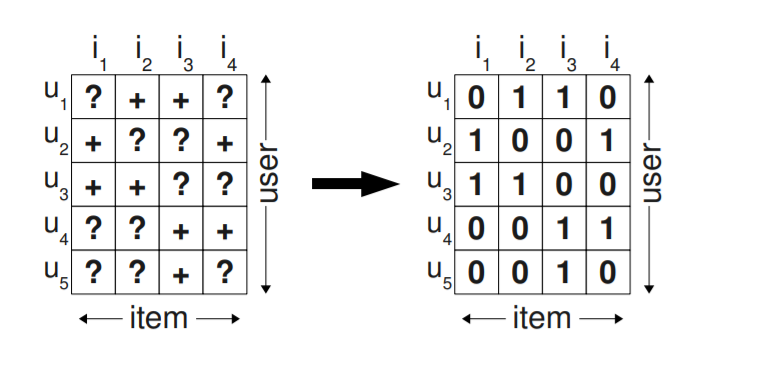
\includegraphics{images/BPR1.png}
    }
    
    \caption{
    \label{BPR1}
         }
    \end {center}
    \end {figure}
    Обычный подход заключается в том, чтобы предсказать
     персонализированную оценку для элемента, которая отражает 
     предпочтения пользователя для этого элемента. После этого 
     предметы будут ранжированы на основе этого балла. Здесь,
      как вы можете видеть на рисунке \ref{BPR1}, все существующие 
      взаимодействия между Пользователем и элементом помечаются как 
      положительный класс(1), а остальные взаимодействия помечаются
      как отрицательный класс(0).

      В подходе Байесовского
      персонализированного ранжирования, вместо взятия одного элемента, 
      пары элементов будут рассматриваться как обучающие данные. Оптимизация
       будет выполняться на основе ранжирования этих пар пользователь-элемент,
        а не только на основе взаимодействия пользователя и элемента. Набор
         данных, который будет рассматриваться, сформулирован следующим
          образом 
          \begin{equation}
            (u,i,j) \in D_S
            \label{eq:1}
          \end{equation}
          Семантика (\ref{eq:1}) заключается в том, что пользователь ${u}$, как предполагается, более предпочитает ${i}$, чем ${j}$.
          \begin{figure}[ht]
            \begin{center}
            \scalebox{0.6}{
               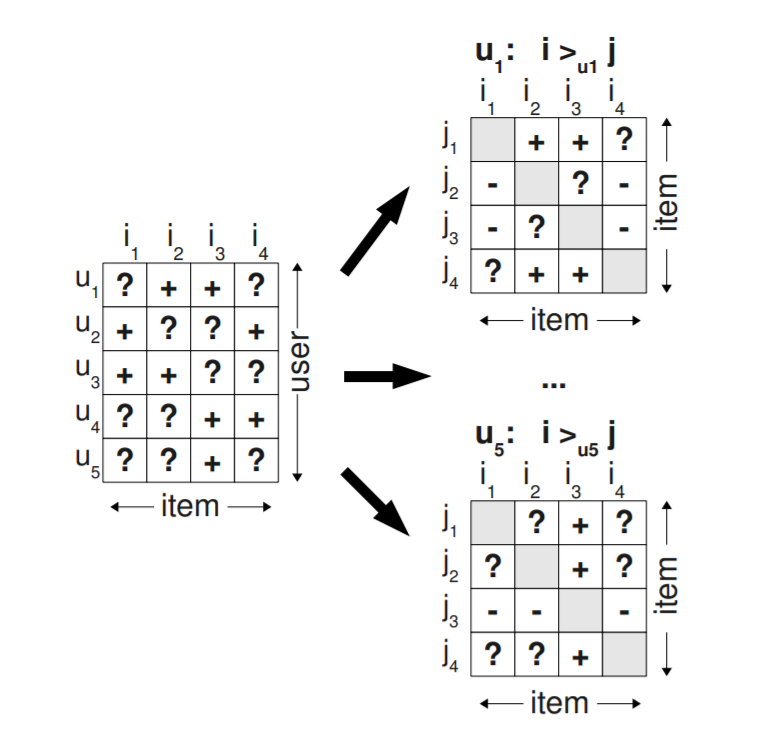
\includegraphics{images/BPR2.png}
            }
            
            \caption{
            \label{BPR2}
                 }
            \end {center}
            \end {figure}

            Здесь триплеты, сгенерированные для обучающих данных, представляют собой специфические для пользователя попарные предпочтения между парой элементов.
            
    На приведенном выше рисунке пользователь ${u_1}$
    просматривал элемент ${i_2}$, но не элемент ${i_1}$,
    поэтому алгоритм предполагает, что этот пользователь 
    предпочитает элемент ${i_2}$ ${i_1}$ ${(i_2 > i_1)}$ и дает положительный 
    знак. Никакой вывод не может быть сделан о предпочтении для элементов, 
    которые были замечены пользователем и показаны как отметка $?$. То же 
    самое верно и для двух элементов, которые пользователь еще не видел 
    (например, элемент ${i_1}$ и ${i_4}$ для пользователя ${u_1}$).
     Напротив, вы можете наблюдать отрицательный знак для ${(i_1, j_2)}$,
      поскольку пользователь предпочитает item2 item1.

      Как и в любом байесовском подходе, в этом подходе мы имеем функцию правдоподобия, априорную вероятность и апостериорную вероятность.
      Байесовская формулировка нахождения правильного персонализированного 
      ранжирования для всех элементов ${i \in I}$ заключается в максимизации 
      следующей апостериорной вероятности, где $\Theta$ представляет вектор 
      параметров произвольного класса моделей (например, матричная 
      факторизация).

      \begin{equation}
        p(\Theta| >_u) \propto p(>_u| \Theta)p(\Theta)
        \label{eq:lik}
      \end{equation}

      Функция правдоподобия (\ref{eq:lik}), где ${>_u}$ -- это необходимые, 
      но латентные предпочтения структуры для пользователя $u$.

      Предполагая, что пользователи будут действовать независимо и порядок 
      каждой пары элементов ${(i, j)}$ для конкретного пользователя не зависит 
      от порядка каждой другой пары, мы можем сформулировать индивидуальную 
      вероятность того, что пользователь предпочитает элемент $i$ элементу $j$ 
      следующим образом:
      \begin{equation}
        p(i >_u j|\Theta) := \sigma(\hat x_{uij}(\Theta))
        \label{eq:ver}
      \end{equation}
    где $\sigma$ логистическая сигмоида: 
    \begin{equation}
        \sigma(x) := \frac{1}{1+e^{-x}}
        \label{eq:sigm}
      \end{equation}

${\hat x_{uij}(\Theta)}$ -- это в приведенном выше уравнении (\ref{eq:ver}) является 
вещественной значимой функцией, которая представляет собой отношение 
между пользователем $u$, элементом $i$ и элементом $j$ и обычно вычисляется 
с использованием модели матричного факторизации. Другими словами, баллы, 
отражающие отношение между пользователем u, элементом $i$ и элементом $j$, 
будут рассчитываться с использованием данных триплетного обучения и 
матричного факторизации и завернуты в сигмоидную функцию (\ref{eq:sigm}). Эта сигмовидная 
функция дает индивидуальную вероятность, которая будет оптимизирована в 
ходе процесса.

${p(\Theta)}$ - это априорная вероятность, представляющая собой нормальное 
распределение с нулевым средним и дисперсионно-ковариационной матрицей.
\begin{equation}
    p(\Theta) \sim N(0, \Sigma_{\Theta})
    \label{eq:apr}
  \end{equation} 

  Следующее уравнение (\ref{eq:opt}) является окончательным критерием Байесовского
  персонализированного ранжирования, который должен быть оптимизирован
  \begin{equation}
    \sum_{(u,i,j)\in D_S} \ln \sigma(\hat x_{uij}) - \lambda_\Theta||\Theta||^2
    \label{eq:opt}
  \end{equation} 
  где $\lambda_\Theta$ -- специфические параметры регуляризации модели.

  \subsection{Реализация на языке программирования Python}
  Так как предполагается, что данные будут подаваться в файлах фората csv,
  то была выбрана библиотека pandas \cite{pandas} для работы с данными.
  Данные представлены в формате id пользователя, id элемента, оценка 
  элемента пользователем, класс, к которому принадлежит элемент.
  Выбирается порог оценки элемента, выше которого оценка считается положительной.
  Для дальнейшей работы представляем данные в виде разряженной таблицы, для более быстрой работы с большими таблицами.
  Из библиотеки Implicit \cite{imp} и метода BayesianPersonalizedRanking
   берем реализацию Байесовского
  персонализированного ранжирования.
  Разделяем исходные данные на тренировочную и тестовую выборки, 80\% даннхы на 
  тренировочную и 20\% на тестовую. На тренировочной выборке строим алгоритм рекомендаций.

  Далее реализуем метрики для проверки качества полученных рекомендаций.
  В качестве метрики для проверки точности рекомендаций используем precision (\ref{eq:prec}) (точность),
  а в качестве метрики сравнения исходного распределения и полученного, будем использовать
  дивергенцию Кульбака-Лейблера (\ref{eq:KL}). Для проверки будем брать
  30 лучших рекомндаций для пользователя.

  Калибровку рекомедаций будем производить двумя методами: первый (\ref{eq:Calibrated})
  основан на дивергенции Кульбака-Лейблера, а второй является 
  адаптацией метода Сент-Лагю \cite{bib5}.

Для визуализации результатов используется библиотека Matplotlib \cite{plot},
с помощью нее строится график распределения классов рекомендованных 
элементов, для сравнения реального, сгенерированного рекомендательной системой 
и откалиброванного распределений.

Для сравнения с готовым решением будем использовать фреймворк SurPRISE \cite{sur} на языке программирования Python.
Из набора реализованных во фреймворке методов используем основанный на предположении о нормальном распределении NormalPredictor.

Алгоритм прогнозирования случайной оценки основан на распределении обучающего множества, которое принято считать нормальным.
Предсказание ${\hat r_{ui}}$ формируется из нормального распределения ${\mathcal{N}(\hat{\mu}, \hat{\sigma}^2)}$,
где ${\hat \mu}$ и ${\hat \sigma}$ оцениваются из обучающих данных, используя оценку максимального правдоподобия:

\begin{equation}
  \hat{\mu} = \frac{1}{|R_{train}|} \sum_{r_{ui} \in R_{train}} r_{ui}
\end{equation} 
\\
\begin{equation}
  \hat{\sigma} = \sqrt{\sum_{r_{ui} \in R_{train}} \frac{(r_{ui} - \hat{\mu})^2}{|R_{train}|}}
\end{equation}